\documentclass{article}[10pt]
\usepackage[utf8]{inputenc}
\usepackage[english]{babel}
\usepackage[margin=0.8in]{geometry}
\usepackage{graphicx}
\graphicspath{{images/}}
\usepackage{multicol}

\author{
  Héctor Otero Mediero\\      \texttt{hoterome@uci.edu}
  \and
  Nikita Samarin\\      \texttt{nsamarin@uci.edu}
}
\title{Lip Reading}

\begin{document}
\maketitle

\begin{multicols}{2}

\section{Introduction}
Lip Reading is one of the tasks which is equally hard both for humans and machines,
but it can be potentially used in a wide range of applications. Lip reading can
provide aid to hearing-impaired people by helping them understand what others are
saying. It can improve general-purpose voice recognition systems, especially in
noisy environments, and can enable silent dictation in public areas. Other
applications include silent film annotation and improved automatic subtitle
generation, for instance on YouTube.
\section{Description of the Problem}
Lip reading is the task of decoding text from the movement of a speaker’s mouth,
often in situations where normal sound is not available. Solving this problem
would mean going from video footage of someone speaking with their lips visible
to the actual text being pronounced, without using any sound data. Accurately
performing such classification over large vocabularies is a hard task.
Last year, researchers from Google DeepMind division managed to achieve accuracy
of 46.8\% on BBC corpora consisting of 17500 words. At the same time, however,
a professional lip-reader managed to annotate only 12.4\% of words without any error [1].
In our project we focused on a limited vocabulary, performing classification of short phrases,
as opposed to single words or complete sentences. Simplifying the problem gave us more time
for data preprocessing and different neural network models prototyping.
\section{Previous Work}
In recent years, there has been a significant number of works which utilize deep
learning to solve problems in the field of speech processing and image recognition.
Lip reading is not an exception, as neural networks achieve higher accuracy
than earlier models that rely on heavy preprocessing of frames and video feature
extraction. Chung \& Zisserman (2016a) propose a two-stream convolutional neural
network (CNN) architecture to determine the audio-video synchronization between
mouth motion and speech in a video [2]. They apply the network to lip reading
and manage to achieve 91.4\% accuracy for 10-phrase classification on the OuluVS2
dataset. Chung \& Zisserman (2016b) focus exclusively on Lip Reading for which
they develop CNN architectures that can learn and recognize words from video
frames collected from TV broadcasts [3]. They train the model on the BBC TV
dataset and obtain 93.2\% accuracy on OuluVS2. Of greater importance, however,
is LipNet – first end-to-end sentence-level lipreading model developed by
researchers from University of Oxford and Google DeepMind department [4]. The
architecture of the model is composed of spatiotemporal CNNs and bidirectional
gated recurrent units with connectionist temporal classification as the loss
function. On the GRID corpus, LipNet achieves 95.2\% accuracy in sentence-level
classification problem.
\section{Dataset}
Solving lip reading problem is notorious for the fact that there are only few
comprehensive datasets with sufficient number of training examples. For our
project, we contacted University of Oulu in Finland in order to obtain OuluVS
database [5]. It includes the video and audio data for 20 subjects uttering
ten phrases: Hello, Excuse me, I am sorry, Thank you, Good bye, See you, Nice to
meet you, You are welcome, How are you, Have a good time. Each person spoke each
phrase five times. There are also videos with head motion from front to left,
from front to right, without utterance, five times for each person. Frame size
for each video is 576x720 with 25 frames per second. We attempted to retrieve
other popular datasets, such as GRID and BBC corpora, but we were not provided
access to them.\\

Before we could perform lip reading, we first had to build a model to locate the
lips on an image. The videos in our dataset did not provide sufficient number of
frames to train such model, therefore we consulted additional face databases, such
as Richard's MIT database (924 images of size 480x640) and Yale Face Database
(165 images of size 320x243) [6]. We used dlib Image processing library to
generate training data for these images, by locating the mouth on the image and
outputting coordinates of the surrounding box to a csv file.\\

At the same time, we also wanted to create a model to analyze sound data from
videos, so that we could potentially improve our lip reading predictions. For
this purpose, we used FFmpeg tool to extract wav audio files from the video
recordings of the OuluVS dataset.

\section{Hardware}
Macbook Pro: 2.4GHz dual-core Intel Core i5 processor, 8GB DDR3L, 256GB\\
Windows 10 PC: 2.8GHz dual-core Intel Core i7 processor, 8.00GB Dual-Channel DDR3, 512GB

\section{Technical Approach}
\subsection{Using video frames}

Our first attempt at tackling the problem followed a pure lip reading approach,
this is, using only a sequence of still images (video frames) from a subject to
predict the sentence that is said in the video. Previous works in the field used
3D Convolutional Neural Networks to process the sequence of images with
successful results, but our hardware did not fit well to this task, as the
computational requirements are high and a single epoch for
processing 500 videos took around 2 hours. Due to the impossibility of following this path, we
flattened the input to be able to process each image as a 1D vector and be able
to feed it into a Recurrent Neural Network or a 2D convolutional Network
(after forming a matrix with all the different frames). The results were not
ideal, as the dimensions of the individual images were too big in comparison with
the amount of examples, yielding networks with too many parameters that
overfitted the data.

\paragraph{Lip Segmentation} ~\\

In order to reduce the dimensionality of the data, we decided to limit the
section of the photo used as input. Obviously, the bulk of the
information stored in an image comes from the mouth of the subject and since the
space it occupies is rather small in comparison with the image size it does a
great job at condensing the information and reducing the amount of parameters in
the network.\\

Since solving image segmentation problems using Neural Networks has been
thoroughly studied, we designed our own. The problem at hand was finding the
coordinates of the top left corner and the width and height of a bounding box
that surrounded the subject's mouth. The dataset we were working with included
labeled data of each one of the frames extracted from the videos with this
information. \\

As it can be seen in the image below the architecture used is composed by alternating
2D Convolutional layers with MaxPooling2D layers and a final Dense layer that
completes the regression task by predicting 4 values from each image. The
intuition behind this architecture is that, as in Visual Computing techniques,
the convolutional layers will be used to extract features at different levels of
detail and the pooling layers help at reducing further the dimensionality of the
image. Finally, the dense layer with a linear activation produces an unbounded
value, ideal for the regression task.\\

\includegraphics[width=0.8\linewidth,keepaspectratio]{convolution.png}

The results obtained are really accurate. After 25 training epochs and using 80\%
of the data for training and the rest for test, we obtain a Mean Squared Error of
95. The meaning of this error for our case is that, on average, predictions
for the coordinates of the box and the labeled data differ in only 9 pixels, which
for a 576x720 images represents less than 2\% of the width and height.\\

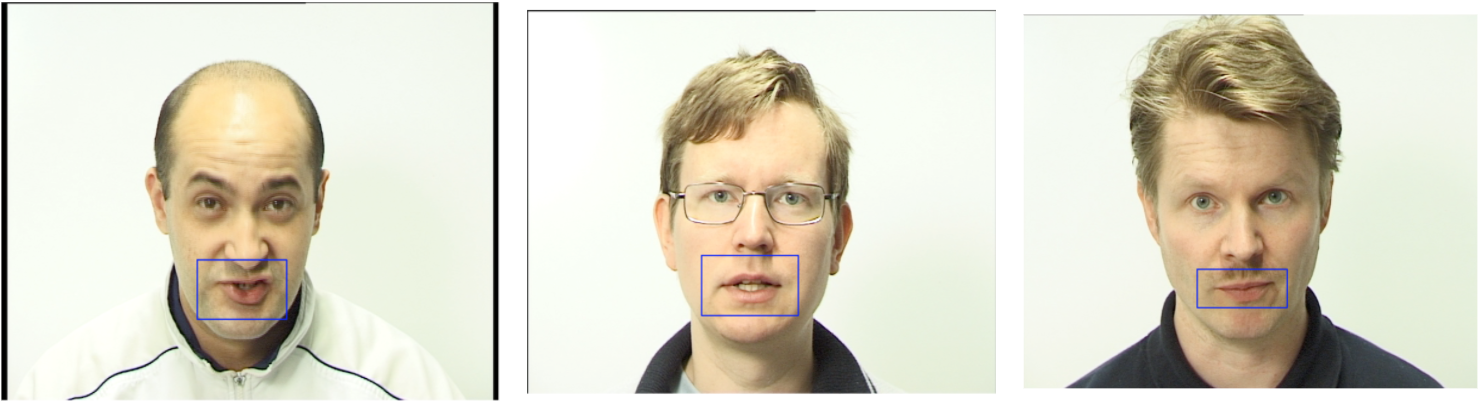
\includegraphics[width=0.8\linewidth, keepaspectratio]{boxes.png}

Some of the reasons behind this accurate prediction are the availability of a
large set of images to work with and the fact that the mouths are centered along
the X-axis.

\paragraph{RNN Architecture} ~\\

Using the previous information to crop the images, we tried feeding them to a
recurrent neural network, considering the fact that there is a relation among the
images that can be expressed as a sequence.  Since we are dealing with a
classification task, we use a Dense layer at the top with a softmax activation
function that returns values for different classes that can be interpreted
as the probability of an example belonging to a certain class.\\

Both types of RNNs available in Keras, LSTMs and SimpleRNNs, were used to test
whether there was a need for establishing a relation between values distant in
the video sequence. The architecture that yielded the best results used the
latter and is shown below. The layer configuration reflects the scarcity of
the data (just 1000 videos), which forced us to constrain our network to a small
amount of parameters, and the subsequent need to avoid overfitting, which led us
to include dropout layers after each of the recurrent ones and try different
types of regularization (L2 with a value of 0.01 providing the best
performance).\\

\includegraphics[width=0.8\linewidth, keepaspectratio]{rnn.png}


The results obtained barely improved a random classification of the data with a
16\% accuracy using categorical crossentropy as loss function for the model. We
think that a solution could be found using this method due to the semantic
relation between the images as explained previously, but recurrent networks that
can process this kind of data need a lot of parameters and, in our case, the
relation with the amount of input data was far from ideal. 2D Convolutional
networks were also tested but they produced worse results.

\subsection{Using video sound}

Due to the poor results obtained using just images, we decided to try solving
the same problem (going from a video to the sentence said) but using the sound
instead, since in most cases where lip reading can be used, sound is available
too (even if it is present with noise). Intuitively, the same information is
stored both in the video and in the sound, the second one being more dense and
simpler than the first.

\paragraph{Data Preprocessing \& Augmentation} ~\\

In order to reduce the problems found with the previous approach, we opted to
increase the amount of training examples. The audio present in the videos was
noisy so we tried different approaches to lessen the effects that they could
provoke in our network, generating new audios by applying a rolling-mean filter
on the audio with a window size of 10 making reducing the noise effectively.\\

Apart from the noise, we tested different representations of the data, integer
and floating point, and a different number of channels, stereo or mono, choosing
in both cases the second option as it produced better results.

\paragraph{CNN Architecture} ~\\

Facing again a vector representation of our input data (in this case
amplitude values for the audio) we could again choose between a recurrent or a
convolutional approach. With our data representation, we saw that audios only
differed one from another on the amount of words pronounced and in terms
of amplitude they were hardly separable. Because of this we chose convolutional
layers as they treat the complete vector instantaneously and could obtain they
aforementioned features better than a recurrent network. \\

Using a layer structure (Figure X) similar to the one built to predict the
bounding box but this time using 1D Convolution we obtained our best results at
predicting the phrase said in a video, a 35\% accuracy. The activation function
for the hidden layers was ReLU as it showed a faster convergence than the rest
and the Adam (Adaptive Moment Estimation) optimizer stabilized the reduction of
the loss in comparison to other optimizers that did not stop the loss from
increasing and decreasing greatly in the validation set.

\section{Conclusions \& Future Work}
We convinced ourselves that performing accurate lip reading is a challenging
problem. While we did not manage to obtain outstanding results, we certainly
managed to identify the weak points of our model design. One of the issues, as
was mentioned above, was our inability to get hold of a bigger dataset. A large
corpus, such as the BBC TV one, would provide significantly more training examples
and improve the accuracy of our model. A logical next step would also be a
combination of our separate models for sound and video frames into a single
ensemble, which would combine the weaker learners into a single stronger one.
Additionally, we did not have access to sufficient computational resources to
try out more complicated models, such as 3D Convolutional Neural Network.
Overall, we created a solid foundation for a future exploration of this problem,
which we will definitely make use of in our subsequent work in this area.

\section{References}
[1] Daily News. Google’s DeepMind AI can lip-read TV shows better than a pro. 2016.\newline
[2] J.S. Chung and A. Zisserman. Out of time: automated lip sync in the wild. In Workshop on Multi-view
Lip-reading, ACCV, 2016a.\newline
[3] J.S. Chung and A. Zisserman. Lip reading in the wild. In Asian Conference on Computer Vision, 2016b.\newline
[4] Y.M. Assael, B. Shillingford, S. Whiteson and N. Freitas. LipNet: end-to-end sentence-level lipreading.
Under review as a conference paper at ICLR 2017.\newline
[5] G. Zhao, M. Barnard and M. Pietikäinen. Lipreading with local spatiotemporal descriptors.
IEEE Transactions on Multimedia 11(7):1254-1265, 2009.\newline
[6] Massachusetts Institute of Technology. Face Databases.
\end{multicols}
\end{document}
